\documentclass[12pt,a4paper]{beamer}
\usepackage[utf8x]{inputenc}
\usepackage{ucs}
%\usepackage[english]{babel}
\usepackage[german]{babel}
\usepackage{amsmath}
\usepackage{amsfonts}
\usepackage{amssymb}
\author{Michael Haas, haas@cl.uni-heidelberg.de}
\title{Johns \& Jones: Construction in Semantic Memory: Generating Perceptual Representations with Semantic Similarity}
\subtitle{Seminar: Multimodale Semantik (Dr. ric. Gerhard Kremer)}
\date{21-05-2013}
\begin{document}


\begin{frame}
\maketitle
\end{frame}

\begin{frame}{Overview}
\begin{itemize}
\item Idea \& Approach %- Dist. Semantics, PSS, Perceptual Simulation
\item Background PSS
\item Data
\item Evaluation
    \begin{itemize}
    \item Model Foundations
    \item Behavioral Simulations
    \end{itemize}
\item Recap \& Discussion
\item \textbf{Questions? Too fast? Ask!}
\end{itemize}
\end{frame}


\begin{frame}{Idea \& Approach}
\begin{itemize}
\item Given
    \begin{itemize}
    \item Linguistic representation for \textbf{all} words
    \item Perceptual representation for \textbf{some} words
    \end{itemize}
\item Learn
    \begin{itemize}
    \item Perceptual representations for \textbf{all} words
    \item Integrated model of linguistic and perceptual information
    \end{itemize}
\item Motivated by Perceptual Systems Theory of knowledge
\end{itemize}
\end{frame}

\begin{frame}{Perceptual Systems Theory}
\begin{itemize}
\item Cognition is inherently perceptual (Barsalou, 1999) %\cite{barsalou}
\item Cognition is grounded in real-world experiences
\item Perceptual systems in the brain perform cognitive functions
\item No separate cognitive and perceptual systems
\end{itemize}
\end{frame}



\begin{frame}{Perceptual Systems Theory: Memory/Knowledge}
How does memory/knowledge work?
\begin{itemize}
\item Human perceives an object: vision, audition, haptics, olfaction, gustation, proprioception, introspection
\item \textbf{Perceptual Symbols}: records of neural states that underlie perception (Barsalou, 1999)
\item Memorizing: selected aspects of object are committed to memory
\item Recalling an object: Perceptual Symbols form a \textbf{simulator} in sensory-motor regions
\end{itemize}
\end{frame}

\begin{frame}{Perceptual Systems Theory}
\begin{figure}
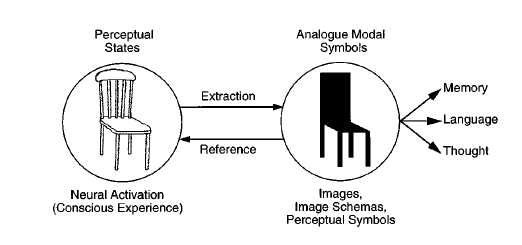
\includegraphics[scale=0.8]{barsalou_figure_1_perceptual_symbol_systems.png}
\caption{Basic idea of Perceptual Systems Theory, \cite{barsalou}}
\end{figure}
\end{frame}


\begin{frame}{Perceptual Systems Theory: Properties of Symbols}
Properties of Perceptual Symbols
\begin{itemize}
\item Can be multi-modal
\item Selective attention: schematic memory, no full reproduction
\item Dynamic, may be changed by new experiences
\item Componential
\item Does not necessarily represent specific individuals
\item Can be indeterminate
\end{itemize}
\end{frame}


\begin{frame}{Perceptual Systems Theory: Amodal theories }
Amodal Theories ($\neq$ Perceptual Symbol Systems)
\begin{itemize}
\item Based on developments in logics, statistics, programming languages
\item Perceptive and cognitive representations happen in different brain regions and systems
\item Perception is transducted into different representative structure, then stored
\end{itemize}
\end{frame}

\begin{frame}{Perceptual Systems Theory: Amodal theories}
\begin{figure}
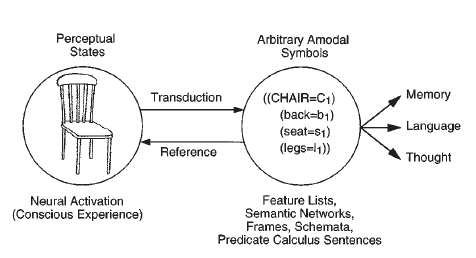
\includegraphics[scale=0.8]{barsalou_figure_2_amodal_symbol_systems.png}
\caption{Basic idea of Amodal theories, \cite{barsalou}}
\end{figure}
\end{frame}

\begin{frame}{Perceptual Systems Theory: Amodal theories}
Problems with Amodal Theories
\begin{itemize}
\item Do not successfully implement spatio-temporal processing
\item No grounding: amodal symbol processing is entirely syntactic
\item Offer no predictions for phenomena, only post-hoc explanations
\item Too powerful, thus unfalsifiable
\end{itemize}
\end{frame}


\begin{frame}{Perceptual Systems Theory and Computational Semantics}
\begin{itemize}
\item Perceptual Systems Theory of knowledge tells us that perceptions and their simulation are the basis for knowledge representation
\item No additional representation needed
\end{itemize}
$\to$ Add perceptual features to semantic model!
\end{frame}

\begin{frame}{Overview}
\begin{itemize}
\item Idea \& Approach
\item Perceptual Systems Theory
\item \textbf{Data}: Linguistic \& Perceptual
\item Evaluation
    \begin{itemize}
    \item Model Foundations
    \item Behavioral Simulations
    \end{itemize}
\item Recap \& Discussion
\end{itemize}
\end{frame}



\begin{frame}{Data: Linguistic data set}
\begin{itemize}
\item Words represented as binary co-occurrence vectors
\item Co-occurence counted across documents
\item Extracted from 250,000 Wikipedia articles
\end{itemize}
\end{frame}


\begin{frame}{Data: Perceptual data set}
\begin{itemize}
\item Probability vectors over perceptual features
\item Generated by \textbf{humans}
\item Not restricted to perception:
    \begin{itemize}
    \item taxonomic features
    \item situational features
    \end{itemize}
\item Different data sources:
    \begin{itemize}
    \item feature generation norms (McRae et al, 2005)
    \item modality exclusivity norms (Lynott \& Connell, 2009)
    \end{itemize}
\end{itemize}
\end{frame}

\begin{frame}{Data: Full lexical representation}
\begin{itemize}
\item Concatenation of linguistic + perceptual data set
\end{itemize}
\begin{figure}
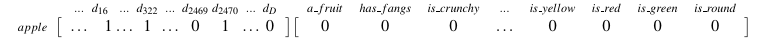
\includegraphics[width=\textwidth]{silber_lapata_example_lexical_representation_figure_3.png}
\caption{Figure by Silberer \& Lapata (2012)}
\end{figure}
\end{frame}


\begin{frame}{Approach: Inference}
$$ Perc_{j} = \sum_{i=1}^{M}{T_{i} \times S(T_{i}, T_{j})^{\lambda} } $$
% M: size of lexicon, T lexical trace, S similarity function (cosine), $\lambda$ similarity weighting parameter
\begin{itemize}
\item Step 1: Only Calculate $Perc$ for words with zero perceptual vector
\item Step 2: (Re)-Calculate $Perc$ for all words
    \begin{itemize}
    \item perceptual features are inferred via global similarity to all lexical entries
    \item aggregation of linguistic and perceptual information from step 1
    \end{itemize}
\end{itemize}
$\to$ Make predictions about perceptual properties/features of words (from global similarity structure)
\end{frame}

\begin{frame}{Approach: Inference}
\begin{figure}
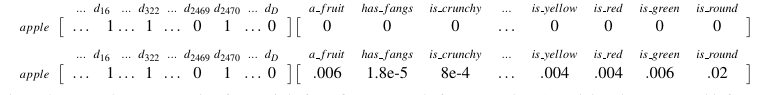
\includegraphics[width=\textwidth]{silber_lapata_example_lexical_representation_and_inference_figure_3.png}
\caption{Figure by Silberer \& Lapata (2012)}
\end{figure}
\end{frame}


\begin{frame}{Overview}
\begin{itemize}
\item Idea \& Approach 
\item Perceptual Systems Theory
\item Data
\item \textbf{Evaluation}
    \begin{itemize}
    \item Model Foundations
    \item Behavioral Simulations
    \end{itemize}
\item Recap \& Discussion
\end{itemize}
\end{frame}




\begin{frame}{Evaluation}
\begin{itemize}
    \item Model Foundations
        \begin{itemize}
        \item How do model parameters affect performance?
        \end{itemize}
    \item Behavioral Simulations
        \begin{itemize}
        \item Does the approach model behavioral phenomena from grounded cognition?
        \end{itemize}
\end{itemize}
\end{frame}

\begin{frame}{Evaluation: Foundations: Word norms}
\begin{itemize}
\item How well does inference of perceptual representation work?
\item Cross-Validation procedure
\item Measure: correlation between inferred and actual perceptual representation
% TODO: What actual correlation measure is used?
\end{itemize}
% Model predictions for each Word Norm
\begin{table}
    \begin{tabular}{lll}
    Word Norm          & Step 1 & Step 2 \\
    McRae, et al.      & 0.42   & 0.72   \\
    Vinson \& Vigglioco & 0.42   & 0.77   \\
    Lynott \& Connell   & 0.83   & 0.85   \\
    \end{tabular}
\end{table}
\end{frame}

\begin{frame}{Evaluation: Foundations: Lexicon Size}
\begin{itemize}
\item What is the effect of lexicon size on inference quality?
\item Use $2000 \to 24000$ most frequent words
\item Result: noise accumulation reduces model performance
% TODO: frequency distribution not provided, compare Zipf?
\item Rough estimate: rank 1: 10**8, rank 10000: 10000\footnote{http://imonad.com/seo/wikipedia-word-frequency-list/, accessed 2013-06-17}
\end{itemize}
\begin{figure}
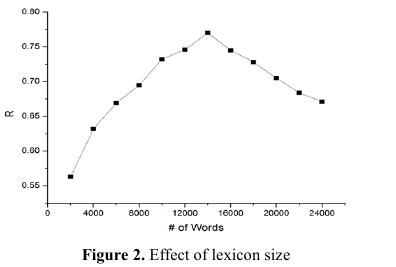
\includegraphics[scale=0.8]{figure_2_effect_of_lexicon_size.png}
\caption{Effect of lexicon size on inference quality}
\end{figure}
\end{frame}


\begin{frame}{Evaluation: Foundations: Effect of Corpus Size}
\begin{itemize}
\item How does corpus size affect inference quality?
\item Model trained on
    \begin{itemize}
    \item Wikipedia Corpus, n=250,000: $r = 0.77$
    \item TASA corpus\footnote{Zeno, S., Ivens, S., Millard, R., \& Duvvuri, R. (1995).The educator’s word frequency guide. Touchstone Applied Science Associates (TASA), Inc.}, n=37,600: $r = 0.64$
%
%  10 million words of UNMARKED high-school level English text on
%  Language arts, Health, Home economics, Industrial arts, Science,
%  Social studies, and Business.
%
    \end{itemize}
\item Result: increasing number and diversity of contexts improves performance
% "the greater the amount of experience the model has with language, the better its inferences
%are about a word's perceptual representation"%
\end{itemize}
\end{frame}

\begin{frame}{Evaluation: Foundations: Reverse Inference}
\begin{itemize}
\item Can the model infer linguistic distribution from perceptual information?
    \begin{itemize}
    \item Infer ''forward'' perceptual data from linguistic data
    \item Infer reverse linguistic data from learned perceptual data
    \end{itemize}
\item Measure: correlation between inferred co-occurence vector and original
\item For nouns by McRae, et al $r = 0.67$
\item Rest $r = 0.5$
%Reasons: 1) perceptual space does not extend to all words, 2) abstract words%
\item Result: Lexical inferences possible in both directions
\end{itemize}
\end{frame}


\begin{frame}{Overview}
\begin{itemize}
\item Idea \& Approach 
\item Perceptual Systems Theory
\item Data
\item Evaluation
    \begin{itemize}
    \item Model Foundations
    \item \textbf{Behavioral Simulations}
    \end{itemize}
\item Recap \& Discussion
\end{itemize}
\end{frame}


\begin{frame}{Evaluation: Behavioral: Affordance}
\begin{itemize}
\item ''Hang the coat on the --------''
    \begin{itemize}
    \item ''coat rack'' - \textbf{realistic}
    \item ''vacuum cleaner'' - \textbf{afforded}
    \item ''cup'' - \textbf{non-afforded}
    \end{itemize}
\item Can the model replicate human affordance judgment?
\end{itemize}

\end{frame}



\begin{frame}{Evaluation: Behavioral: Affordance}
\begin{itemize}
\item Experiment: calculate cosine similarity between central action word and objects for
\item Example: Calculate
    \begin{itemize}
    \item $sim(hang,rack)$
    \item $sim(hang,cleaner)$
    \item $sim(hang,cup)$
    \end{itemize}
\item on
    \begin{itemize}
    \item inferred perceptual vectors
    \item raw co-occurrence vectors
    \end{itemize}
\item Desired: $sim(hang,rack) > sim(hang,cleaner) > sim(hang,cup)$
\end{itemize}
\end{frame}



\begin{frame}{Evaluation: Behavioral: Affordance}
\begin{figure}
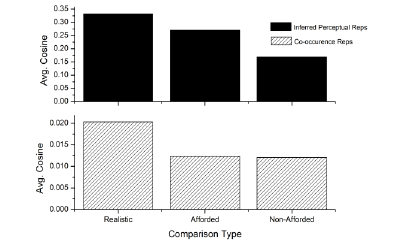
\includegraphics[scale=0.7]{figure_3_affordance_distinction.png}
\caption{Inferred affordance ratings}
\end{figure}
\begin{itemize}
\item Result: inferred perceptual vectors provide better distinction between affordance ratings
\end{itemize}
\end{frame}



\begin{frame}{Evaluation: Behavioral: Sensory/motor based priming}
% Neural facilitation in neuroscience, is the increase in postsynaptic potential evoked by a 2nd impulse. %
Sensory/motor based priming
%TODO: re-formulate, start with example%
\begin{itemize}
\item Original experiment: priming based on common sensory-motor information leads to facilitation
\item Facilitation: increased synaptic potential by a second impulse
\item Related-Target: ''piano'' $\to$ ''typewriter''
\item Unrelated-Target: ''cheese'' $\to$ ''typewriter''
\item No associative information between words
\item Focus on manipulation knowledge
\item $\to$ Significant faciliation found for human subjects
\end{itemize}
\end{frame}

\begin{frame}{Evaluation: Behavioral: Sensory/motor based priming}
\begin{itemize}
\item Experiment: compare similarity in model between related-target and unrelated-target
\item Measure: $sim(related,target) - sim(unrelated,target)$ as magnitude of facilitation
\item Result: model successfully infers perceptual information
\end{itemize}
\end{frame}

\begin{frame}{Evaluation: Behavioral: Sensory/motor based priming}
\begin{figure}
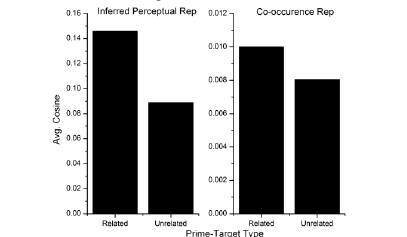
\includegraphics[scale=0.7]{figure_4_perceptual_priming_results.png}
\caption{Simulation of perceptual priming results}
\end{figure}
\begin{itemize}
\item Difference not significant for raw co-occurrence representations
\item Difference significant for inferred perceptual representations
\end{itemize}

\end{frame}


\begin{frame}{Evaluation: Behaviorial: Phrase/referent similarity}
Phrase/referent similarity
\begin{itemize}
\item Data set: novel and familiar noun phrases 
\item Familiarity rated by test subjects
    \begin{itemize}
    \item Novel: ''smashed tomato''
    \item Familiar: ''sliced tomato''
    \end{itemize}
\item Can model account for human similarity ratings?
\end{itemize}
\end{frame}

\begin{frame}{Evaluation: Behaviorial: Phrase/referent similarity}
\begin{itemize}
\item Measure: ''familiarity'' computed as cosine between two words
\item Desired: $sim(sliced,tomato) > sim(smashed,tomato)$
\item Marginally significant difference between novel and familiar condition
\item But: significant correlation between computed familiarity and subject ratings on item level for inferred perceptual representations
\item Result: model can simulate
    \begin{itemize}
    \item phrase familiarity - how often subjects had experienced specific phrase
    \item referent familiarity - how often subjects had seen specific object
    \end{itemize}
\end{itemize}
\end{frame}

\begin{frame}{Evaluation: Behavioral: Inferred Modality Representation}
Inferred Modality Representation
\begin{itemize}
\item Perception has five modalities: visual, auditory, tactile, olfactory, gustatory
\item Modalities can be dominating for concepts and properties
\begin{itemize}
    \item \textbf{yellow}: visual
    \item \textbf{rustling}: auditory
    \item \textbf{round}: visual, haptical -- multimodal
\end{itemize}
\item Modality exclusivity norms released by Lynott \& Connell (2009) \cite{lynott} 
\end{itemize}
\end{frame}

\begin{frame}{Evaluation: Behavioral: Inferred Modality Representation}
\begin{itemize}
\item Words represented as probability distribution over five modalities
\item Experiment:
    \begin{itemize}
    \item Take word with known dominant modality
    \item Set up model with modality norms instead of feature norms (drawing from additional data sets)
    \item Infer modality norms for selected word
    \item Compare against random sample from different modality
    \end{itemize}
\end{itemize}
\end{frame}

\begin{frame}{Evaluation: Behavioral: Inferred Modality Representation}
\begin{figure}
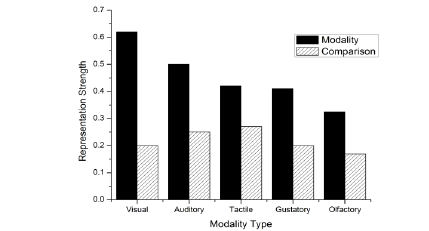
\includegraphics[scale=0.7]{figure_5_level_of_strength_for_different_modalities.png}
\caption{Result: Correct inferences about modality basis of words}
\end{figure}
\end{frame}



\begin{frame}{Recap}
\begin{itemize}
\item Simple model integrating linguistic and perceptual data
\item Allows inference of perceptual vectors from incomplete data via global lexical similarity
\item Based on Perceptual Systems Theory
\item Allows integration of various perceptual data sources
\end{itemize}
\end{frame}


\begin{frame}{Thoughts \& Discussion}
\begin{itemize}
\item Joint learning instead of vector concatenation?
\item Acquisition bottleneck for perceptual data
\item How useful are correlation values $0.75$?
\item Cut-Off for word frequency too low?
\end{itemize}
\end{frame}




\begin{frame}{References}
\begin{thebibliography}{-}
% APA
\bibitem{jj} Johns, B. T., \& Jones, M. N. (2011). Construction in semantic memory: Generating perceptual representations with global lexical similarity. In Expanding the space of cognitive science: Proceedings of the 33rd Annual Meeting of the Cognitive Science Society (pp. 767-772).
\bibitem{lynott} Lynott, D., \& Connell, L. (2009). Modality exclusivity norms for 423 object properties. Behavior Research Methods, 41(2), 558-564.
\bibitem{mcrae} McRae, K., Cree, G. S., Seidenberg, M. S., \& McNorgan, C. (2005). Semantic feature production norms for a large set of living and nonliving things. Behavior Research Methods, 37(4), 547-559.
\bibitem{silberer} Silberer, C., \& Lapata, M. (2012, July). Grounded models of semantic representation. In Proceedings of the 2012 Joint Conference on Empirical Methods in Natural Language Processing and Computational Natural Language Learning (pp. 1423-1433). Association for Computational Linguistics.
\bibitem{barsalou} Barsalou, L. W. (1999). Perceptual symbol systems. Behavioral and brain sciences, 22(04), 577-660.
\end{thebibliography}
\end{frame}
\end{document}
